% Chapter Template

\chapter{Implementation} % Main chapter title
%Possible solutions (in the context)
\label{Chapter4} % For referencing the chapter elsewhere, use \ref{Chapter1} 

After introducing the project as it existed before this thesis,
this chapter will concern the planning and implementation of the extension that was build.
The implementation used the aforementioned tools as well as some smaller libraries that will be explained in the following sections.

\section{Project Design}
The project's design followed the in Chapter \ref{Chapter2} explained "Design Thinking" approach.
The following shows the different steps that were taken that lead to the changes that were planned.

\begin{description}
	\item [Empathise]\hfill \\
	      As a first step, interviews and tests with the existing project were executed.
	      Originally, the author wanted to build another riddle for the room.
	      It was quickly discovered that constraints would complicate that task.
	      Three people who had worked with the room reported they experienced severe difficulties
	      on trying to change the existing pattern.
	      Frequently mentioned was the overall lack of understanding the room as a whole.
	      Some parts, like the TCP-socket in Unity, were relatively easy to modify, others, like the riddles themselves were disclaimed
	      "not to be touched or they might break".
	      As the room had many visitors (a few a hours a day, 2-4 times a week), changes which would affect the look
	      of the room or make it unstable for a longer period of time were not welcomed.

	      In the time following these interviews,
	      a deeper occupation with the project seemed necessary to develop alternative ideas for this thesis.
	      The author's impression was that the project lacked documentation and explanations on many sides.
	      Understanding the processes and the different parts of communication proved to be difficult,
	      as it didn't seem to follow any standardized structure or protocol.
	      The result of this examination is further explained in Chapter \ref{Chapter3}.

	      On questioning the former architect about his choices,
	      he stated that the project was build under time pressure
	      and everything was therefore implemented best to the architect's knowledge,
	      but without further scientific research or extensive planning.

	\item [Define]\hfill \\
	      The "Empathize" stage lead to the impression that a new riddle
	      would be considered "nice-to-have" whereas
		  extensions to improve the flexibility and comprehensibility of the room would be welcomed.
		  Derived from the workload analysis in Chapter \ref{Chapter3},	 
	it was determined that the cognitive and memory work required from a developer were the most critical points
	that one might spend a lot of time on, or might decide not to join the project at all.
	It was defined that:

	To reduce cognitive (C) work, the process of learning and discovering the project must be simplified.

	To reduce the memory (M) work, the amount of commands to remember to control the room must be reduced and the start-up of the room must be simplified.

	\item [Ideate]\hfill \\
	The next step was to devise ideas and to estimate their workload to decide 
	which should be included in the prototype. Since the author had little experience as a software developer,
	complicated coding tasks (judged by the author's supervisor) were cut, 
	like a graph-editor for the front-end.

	After discussing possible approaches, a few specific tasks were set:
	      \begin{enumerate}
		      \item Developing a web interface that would:
		            \begin{itemize}
			            \item Enable more overview and control for the existing riddles (M)
			            \item Ease the testing process for new riddles by displaying them dynamically (C)
			            \item Allow remote access (P) and control (C) within the local WI-FI environment
		            \end{itemize}
		      \item Retrieving information from the room must work automatically, therefore should the "feedback mode" be enabled on start-up (M)
		      \item Providing a thorough documentation for future developers  (C/M)
	      \end{enumerate}

	      The summarized goals for improvement in the different areas can be seen in figure \ref{fig:workload}.

	      \begin{figure}[th]
		      \centering
		      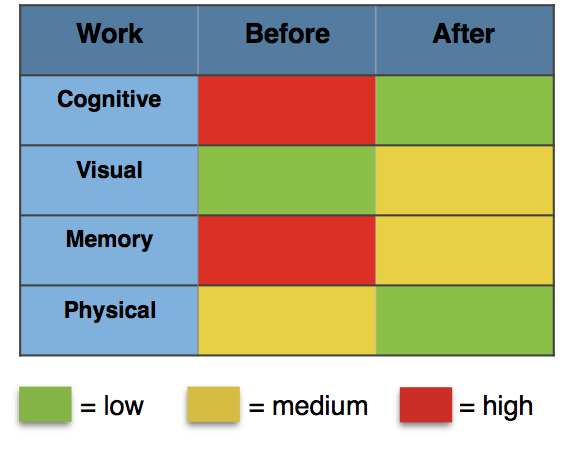
\includegraphics[width=50mm,scale=.5]{Figures/workload}
		      \decoRule
		      \caption[workload]{Workload of the different aspects color-coded}
		      \label{fig:workload}
	      \end{figure}

	\item [Prototype]\hfill \\
		 Afterwards, prototyping began. 
		 The development process of the prototype is explained in the following sections of this chapter.
	    Proof of Concepts were designed for each stage of the implementation (\ref{fig:PoC}).
	\item [Test]\hfill \\
		  Testing happened regularly at least once a month, later every two weeks.
		Extensive testing was difficult to achieve, as the room did not provide 
		   an internet connection needed to install modules (e.g. Node.js) on the PC 
		   and missed basic testing tools like a coding environment. 
		   Additionally, due to the room's physical set-up, testing directly on the PC turned out 
		   to be inconvenient. The PC was hidden behind a wall and difficult to access, 
		   which meant mouse and keyboard could barely reside outside the wall's recess.
		   Consequently, most testing was conducted on two laptops brought by the author: 
		   One Macbook Pro from 2009 with OSX 10.11.6, and a Windows laptop with Windows 10 installed.
		   Throughout testing, new features were designed and iterated.
\end{description}

Our final result is a MVP %Reference abkürzung 
which provides the bare functionalities but lacks in design 
and more extensive features which we will elaborate in the evaluation.

\begin{figure}[th]
	\centering
	\includegraphics[width=100mm,scale=1]{Figures/TablePoc}
	\decoRule
	\caption[Proof of Concept Steps]{List of our PoC steps}
	\label{fig:PoC}
\end{figure}


\section{Architecture}

As happening in other contexts, 
a Service Orientated Architecture (SOA) approach for middleware 
was proposed in many IoT - architectures from the last few years \parencite{archsurv1}. 
SOA encourages decomposition of a complex system into simpler and isolated components.
Thus, reusability and changeability is increased. 
Especially an IoT-scenario with flexible gateway components and on-going extensions can profit from such 
architecture as changes are demanded frequently.
\parencite{archsurv1}

The goals were set with that architecture in mind and resulting architecture changes
designed to become loosely coupled to encourage improving a specific module of the project.
For example, the TCP- and serial-connection were set-up in a general way (send/ receive all) 
to separate the data processing from the transport channels. 
Also, communication was designed not interfere with other each other, e.g. 
communication to Unity should still work if a connection to the front-end failed.
For that reason, a back-end was implemented which ensured reliable data storage.

In that way, changes reflect the composition of a fog architecture, 
though there is no cloud available or planned which is an important part 
of larger IoT project architecture.
The front-end connection received it's own namespace for Socket.io events so front-end relevant data
would only be processed in it's set namespace component.

\begin{sidewaysfigure}
	\centering
	\includegraphics[width=200mm,scale=2]{Figures/escapeUmlNew}
	\caption[New Escape Room Architecture]{The new escape room architecture}
	\label{fig:newEscapeUml}
\end{sidewaysfigure}
%picture of our architecture

\section{Device}
Since the room consisted of microcontroller-driven-riddles only at the time of this thesis, 
we decided to design a prototype and a template for integration of future microcontroller-driven-riddles.
The principle concepts though are applicable to any device.

\subsection{RFM69HCW Wiring}
As most riddles are connected to RFM69HCW-radio- \ transceiver-modules manually, the first set-up of the prototype 
consisted of an Arduino Uno connected to a RFM69HCW. As one can see in figure \ref{fig:prototypeV1},
the wiring looks unorganized.

Later, the set-up was replaced with an Adafruit Feather 32u4 which is a microprocessor with an integrated 
RFM69HCW module an therefore reduces the complexity of the wiring needed for the riddle.
This prototype included an external battery as the Feather doesn't support 5V output.
The Adafruit Feather 32u4 needs an external library to work, the only difference though (apart from the radio set-up)
is the assignment of the SPI lines.

The pictures were drawn with a tool called "Fritzing". 
Fritzing is a popular open-source software for the design of electrical microporcessor-hardware.
It and enables prototyping and e.g. generates circuit diagrams automatically and testing code in an interface. 
To achieve that, someone needs to set the specifications (I/O, behavior) of a part. 
The developed part is called a "Fritzing-part" opposed to a "Fritzing-app" which is a project containing several connected Fritzing-parts. 
Projects can be shared in the Fritzing forum \parencite{fritzingForum}. It was developed by the University of Applied Sciences in Potsdam

\begin{figure}[H]
	\centering
	\includegraphics[width=75mm,scale=.75]{Figures/prototypeV1}
	\decoRule
	\caption[First Version of the Prototype]{Prototype, Version 1}
	\label{fig:prototypeV1}
\end{figure}


\begin{figure}[H]
	\centering
	\includegraphics[width=50mm,scale=.5]{Figures/prototypeV2}
	\decoRule
	\caption[Second Version of the Prototype]{Prototype, Version 2}
	\label{fig:prototypeV2}
\end{figure}

\subsection{Template}

The template was designed to simplify the process of developing a riddle.
The escape room provided in its prior form no support for new riddle-developers.
We decided to modify the existing communication protocol, 
but had to be careful not to impact communication to the existing riddles.

Still, we wanted simplify the communication system for riddle-developers.

The existing communication protocol followed a "string-to-chararray-send" and "receive -chararray-to-string" structure that we applied to the implementation.
In contrast to the existing puzzles though, we decided to separate the code into several parts, named by the functionality they supplied.

%Chararrays are smaller than strings hence faster for radio-communication.
The template is divided into 4 parts: "Groundwork", "Riddlefunctionality","Remote Functionality" and "Radio communication".

\begin{description}
	\item [Groundwork]\hfill \\
	      Section to be filled with libaries, variables and definitions.
	\item [Riddle Functionality]\hfill \\
	      To contain the riddles functionalities (e.g. code activation rules) separated from nearly any communication.
	      The only communication that needs to be defined here is when the microcontroller should send messages and which.
	      That is executed by writing a single line command containing the desired string.
	      If the string's value is defined in the "registerRiddle()" function of the "Remote Functionality" section, it will be translated in the web interface.
	\item [Remote Functionality]\hfill \\
	      To contain any remote commands for interaction with the web interface and the server.
	      The "Remote Functionality" section consists of two functions:
	      \begin{description}
		      \item [registerRiddlle()]\hfill \\
		            Here is where strings to be send once on starting the device are defined.
		            These strings set the configuration of the variables in the web interface.
		            To work, they need to follow a specific structure:
		            \begin{enumerate}
			            \item an index for the riddlevariable (to order the variables)
			            \item a "readonly" or "write" command (to make it static or dynamic)
			            \item the name of the variable (to translate)
			            \item the value of the variable (needs to be converted into a String)
			            \item an optional button value (if it was present, a button would show)
		            \end{enumerate}
					That structure is meant to be applicable for any variable. 
					It is important to name the "Finish"-command that is send when the riddle is solved "Finish" so it will be recognized by the web interface and the color will change to green once the riddle is finished.
		      \item[remoteCommand()]\hfill \\
					Designed to contain processing of incoming messages from the gateway/ server.
		            It iss connected to the radio functionality further down in the code, nevertheless allows the user not to care about how the messages are processed.
					It is handed a "char message[]" and an "int messageLength" variable on call. 
					The message can be used for a "Switch-Case"-handling of data, e.g. a message "1/1234" could trigger case "1" and further processing with the other numbers could happen in the case function, e.g. setting the numbers as a new code for a riddle.
					Since the message always needs to be iterated with the messages's length to transform it to a string, it seemed useful to hand the message's length right with the message, making the code easier to read and work with. 
					The length is recognized in the "radio communication" section of the template and therefore outside the developers point of focus.
		            The developer is advised to use a "Switch-Case" structure like that to define the microcontroller's reactions to radio messages, to keep the processing clean and standardized.
					For any reaction concerning the defined variables, the case should match the index of the variable in order for the buttons within the web interface to work.
					For example, if in "registerRiddle()", a variable named "won" is assigned the index "1" and has a button value, 
					any desired processing happening when clicking the button should happen in case "1", in this case triggering the function that makes the riddle appear as if the riddle was solved/won.
		
	      \end{description}
	\item[Radio communication]\hfill \\
		  The radio communication section contains a "readRadio"-function that interprets incoming chararrays as strings and hands them to the remoteCommand-function in the "Remote Functionality" section.
		  This design closely resembles the protocol the former architect implemented for communication, though naming was changed to increase readability and the length of the chararray is handed as a second variable to the remoteCommand-function.
		  The "rfm69send"-function is also defined in this section, which is responsible for transforming given strings into chararrays and sending them to the defined gateway RFM69HCW.
\end{description}


\begin{figure}[th]
	\centering
	\includegraphics[width=75mm,scale=0.75]{Figures/registerRiddle}
	\decoRule
	\caption[registerRiddle]{"registerRiddle" definition in the Arduino IDE}
	\label{fig:registerRiddle}
\end{figure}

The documentation provided explains the template in further detail.

\section{Back-End}

For this database, PostgreSQL was used as DBMS.
PostgreSQL is a light-weight open-source object-relational database system. 
Companies like Netflix, Spotify or Instagram \parencite{postgresUsers} rely on the flexible database system which allows SQl and noSQL design.
It is easy to set-up and maintain. 

The relational model was implemented for the back-end.
Two tables were enough to fit our needs.
One table manages the location, name and other general information about the riddle displayed in the main view,
whereas the other one is responsible for saving and editing the information displayed in the pop-up window.
The key predicate was the id of the riddle, which was common to both tables.
This separation simplifies database changes, clarifying the tasks happening on the Node.js server.
The Node.js server connects the information when sending to the front-end by assigning the details with the riddle's id to the corresponding riddle.

%Database schema einfügen
\section{Communication}

For this project, a websocket implementation seemed the most fitting option as realtime - communication between several clients would be required.
 
It was decided to use Socket.io for client-middle-ware-communication.
Socket.io is a Javascript-library designed for real-time communication build on top of a websocket-protocol.
It enables a bi-directional communication channel between client and server and offers a fallback mechanism to long polling when websockets are not available.
There are several fallback mechanisms available that are determined dynamically by Socket.io:
\begin{itemize}
    \item Websocket
    \item Adobe Flash Socket
    \item AJAX long polling
    \item AJAX multipart streaming
    \item Forever Iframe
    \item JSONP Polling
\end{itemize}

The server-side of Socket.io is developed  specifically for Node.js whereas for the client different implementations (e.g. .Net, Swift, C++)\parencite{socketioClients} are available.
Once a connections is established it's maintained and uses a diminishing small amount resources to communicate. 
It uses an event-based system where one participant listens and another emits an event. 
Both Client and Server can emit and listen for events.

\subsection{Webserver}
It quickly became apparent that the webserver would use Node.js for middleware and processing functionalities between our client front-end and the \- database-backend 
due to the reasons mentioned in Chapter \ref{Chapter2} and listed below.

Node.js is an open-source, cross-platform, JavaScript \- runtime-environment. 
With 49.6\% it is this years "Most Popular Framework, Library or Tool" on this years Stackoverflow-survey \parencite{stackOverflowSurvey}.
According to Google Trends, interest is rising since 2012\parencite{gogleTrendNode}.
One explanation for that might be that it's written in Javascript. 
The transition for front-end Javascript developers to developing back-end is eased, because they don't have to learn a new language.
It uses an event-driven architecture which operates on a single threaded event loop using non-blocking I/O calls.
Commands use callbacks to signal they are completed or failed. 
A downside is, that it doesn't allow vertical scaling by increasing the number of CPU cores of the machine it is running on. 
On CPU-intensive applications, that might become a problem - but modules like IPC or pm2 can add that functionality \parencite{pm2}.
Node.js commands are non-blocking and execute concurrently or in parallel. 
It's build on the Google V8 JavaScript engine which compiles Javascript to machine code instead of interpreting it in real time. 
There are thousands of open-source libraries and web frameworks available for Node.js. 

The decisive factor for using Node.js in comparison to other middleware and back-end solutions was that it would be easier to develop and understand a webserver written in the same language as the front-end.

As all the website operations were processed on the client-side, Node.js main operation was the database and handling.
The "pg-promise" library \parencite{pg-promise} was used for database integration with PostgreSQL.
Depending on the event emitted by the web interface, database-queries to select, update or delete entries could be triggered.
If the gateway emitted a message, a control mechanism would check if the riddle was known and either add a new riddle, update an existing riddle (if new variables where recognized) or translate the incoming data.

With Socket.io, the client would register whether a front-end or another client would register and forward the needed data from the database.
By namespacing (creating different channels for different clients), we tried to avoid dispensable traffic.
The gateway would receive the changeable ("write") values and send them to the connected riddles.
The front-end would receive the sorted database data in a sorted json fit to the front-ends data-handling.

%Architecture We tried to implement our functionalities as loosely as possibilities, so 
\subsection{TCP/Serial/Socket.IO-Client}
This part of the middleware changed several times during our development process.

Since the front-end allowed a reassignment of the messages that would trigger an event in Unity, 
filtering the incoming serialmessages before they were sent to Unity via TCP was required.
Furthermore would they need to be checked for eventual new riddleinformation or messages to be translated or displayed in the front-end.
Consequently, this part of the middleware would filter relevant "Finish"-serialmessages through a PostgreSQL-database, 
and activate a "checkSerialMessage" function which would decide on further processing.
First was tried to use the existing C++-server for the architecture but it was quickly discovered that understanding and extending the existing code would probably take longer than recreating the features.

Then, because many developers within the faculty were proficient in C\# from Unity development, an implementation the functionalities was tried with a .NET WPF-App.
This proved to be difficult as well, as it required multi-threading and communication between the threads. 
Both are well documented at the MSDN \parencite{MSDN},
however due to the mass of different techniques it was hard to get an overview.
The resulting code was easier than the C++ code, though not comparable to the readability of the Javascript-code of the Node.js implementation.
It took roughly 40 hours to implement the desired functionalities with .NET.

Finally, the  C\# code was revisited and implemented it in Javascript with the existing Node.js-server to compare the workload and readability. 
Additionally, it would be more convenient to have all processing in one place, in one language, than in two.
The same functionalities took about 20 hours to implement, though the author did by then have little experience in Javascript and started the C\# implementation with Unity-C\#-Knowledge.
Programming an async-TCP-server with basic functionalities takes in node.js about 10 lines of code, whereas the C\#-code was about a 100 lines, 
because async-functionalities need to be implemented by hand.
Implementing a serialport communication was easy in both versions, 
but the communication between the different channels seemed more flexible and all in all easier to read and understand.
The async-capabilities of Node.js revealed a tremendous advantage compared to the threading difficulties experienced with the .NET project in this project.
\begin{figure}[th]
	\centering
	\includegraphics[width=100mm,scale=1]{Figures/tableBackend}
	\decoRule
	\caption[Back-end Overview]{Overview of the back-end challenges}
	\label{fig:BackEndTable}
\end{figure}

\section{Front-End}
For this project, React.js was used as a front-end framework. 
React.js will further be called by it's commonly referred name "React".
React was chosen for it's flexible functionalities and it's big community support that outweighs the other two presented front-end solutions.
Angular too has a big community, but supposedly a flatter learning curve.
React is an Open-Source Javascript-library. 
After developing React in 2011, Facebook soon discovered that it's performance was faster than other implementations of its' kind \parencite{benchmarkReact}and made it Open-Source in 2015. 
In this years' Stackoverflow-Survey, React came third in "Most Popular Framework, Library or Tool" \parencite{stackOverflowSurvey} and is the most popular front-end-framework according to this survey. 
This year, over 100,000 developers participated in the survey. 
A lot of libraries are available to support React's infrastructure.
Its main concepts are:

\begin{description}
    \item[Components] \hfill \\
    React motivates its users to write encapsulated components with single responsibilities. Components combine the HTML-markup and Javscript-functionality of a responsibility. 
    They are supposed to increase reusability. 
    \item[Composition] \hfill \\
    The user can reuse and composite elements as he needs to. 
    The isolated components make code easier to maintain. 
    \item[Uni-Directional Dataflow] \hfill \\
            Properties should not be changed in other components, but passed down as read-only variables. 
            React doesn't want children to affect their parent components. That makes maintainability easier, as there's a clear downward structure in a well designed React project.
            If a user needs to pass changes to a parent component, it's executed with callbacks.
    \item[Virtual Dom]\hfill \\
    A Document Object Model (DOM) is a logical structure of documents in HTML, XHTML, or XML formats. 
    Web browsers are using layout engines to transform or parse the representation HTML-syntax into document object model that we can see in a web browser.
    Usually, when one of these elements changes, the whole structure has to be calculated again. 
    React uses a Virtual DOM as a negotiator to enable calculating only the parts that need calculating. That's also possible because of Reacts' isolated component structure.
    \item[JSX] \hfill \\
	Javascript XML (JSX), extends the ECMAScript JavaScript syntax with XML/HTML-like elements.
	It is React's recommended language of choice, though React supports standard Javascript syntax too.
	"The syntax is intended to be used by preprocessors (i.e., transpilers like Babel) to transform HTML-like 
	elements into JavaScript objects that a JavaScript engine will parse" \parencite{jsx2}.
	The JSX-syntax supports React's idea of isolated components, 
	because HTML and Javascript is defined in a single file instead of multiple files.
	JavaScript functionalities between HTML-code can be used by putting them in curly brackets ("{}").
	The generated code runs faster than an equivalent code written directly in JavaScript \parencite{jsx}.
	Most JSX-components in React follow a specific structure that can be seen in below with an example component that resembles the Edit-button in the web interface .
	Usually, a class describing the components functionality is defined.
	In the class, first, a constructor sets the initial internal values like functions and variables used within the class, 
	second, functions are stated, third, the return-function defines what shall be returned and finally the render-function defines what the returned HTML should look like.
\end{description}
\newpage
\begin{lstlisting}
	//Small JSX Component exporting a button that changes looks when it's clicked
	//Importing necessary libaries
	import React, { Component } from "react";
	import { Button } from "reactstrap";
	
	class EditTest extends Component {
	  //Constructor for defining start settings in this.state and binding functions
	
	  constructor(props) {
		//properties given to us by other components are connected with "props"
		super(props);
		//You need to bind a function in the constructor to call it throughout the class
		this.onEdit = this.onEdit.bind(this);
		//This is were our start settings are defined:
		//We want our Edit button to show "off"/false
		this.state = {
		  isEditing: false
		};
	  }
	
	  onEdit(ev) {
		//New State is set
		this.setState( () => ({ isEditing: !this.state.isEditing }));
	  }
		//Here is where our HTML-Markup is designed, in this case just our Edit Button
	  render() {
		//The value of isEditing is called from the state
		const { isEditing } = this.state;
		//Our text is called with this.props;
		//const{text}= this.props.text;
		//Here starts our HTML, Javascript is marked with "{}" brackets.
		return (
		  <div>
			<Button color="info" onClick={this.onEdit}>
			  {isEditing ? "Done Editing?" : "Edit"}
			</Button>
			<p>This is a React render</p>
		  </div>
		);
	  }
	}	
	export default EditTest;	
\end{lstlisting}
\begin{figure}[t]
    \centering
	\includegraphics[width=100mm,scale=1]{Figures/EditExample1}
	\decoRule
	\caption[ReactEx]{Resulting Output of example code}
	\label{fig:resultReact}
\end{figure}

For setting up the front-end, the Create-React-App was used, which provides a front-end build pipeline with Babel and Webpack.
React recommends to start there for single-page applications \parencite{createReactApp}.
It provides a package.json file in which modules and their versions are defined and set.
This prevents unwanted updates so the existing code won't risk becoming deprecated.
The npm packet manager (which is the standard packet manager for Node.js) automatically generates a package-lock.json file which saves the dependency tree in further detail.
For the file-structure, the recommended approach to group by filetype \parencite{reactStructure} in combination with the Create-React-App-structure was used.

Starting out, it was planned to implement a graph-editor to connect riddles in all thinkable ways.
While listing the desired functionalities (Changeable riddleassignments with "Single", "AND" and "OR" connections to the Unity-events) it was decided that a drag-and-drop table would supply most of those functionalities (Changeable assignments, OR connections) without creating a difficult User-Interface.
The React-dnd library \parencite{reactDND} was used to implement the drag-and-drop functionality in React. 
Currently, it is not mobile-optimized since that was thought to be the less popular use case, but adding a mobile implementation for the module is possible.
When a user dropped a riddle into a "Video" field (and saved), the riddle's "Finish"-command would be reassigned on input to the corresponding Video-Trigger-command.
For example, the "Video1" command was originally triggered by "Riddle1".
If a user wanted to make "Riddle2" trigger "Video1", he needed to replace "Riddle1" in the "Video1"-List with "Riddle2".
Whenever "Riddle2" would now signal it's finished, the "Finish"-code of "Riddle1" would be sent to Unity via TCP.
If a Riddle was newly registered, it would be named "NewRiddle" and appear in the "Unassigned Riddles"-List on the web interface.
We designed an "Edit"-function which enabled changing the name of the riddle and deleting it in case it got corrupted (or deleted in real-life).

Another aspect was the popup-window for the riddles. It was planned to show enough information, yet keep it simple.
Consequently, our layout for the popup-window was designed flexibly to adapt to a desirable output depending on the usecase:
Each variable would be displayed in respect to its in the Arduino defined values.
If a variable was set "readonly", but didn't have a button value defined, the information would be listed plainly.
If a variable was set "write", but didn't have a button value defined, the information would be listed plainly.
Additionally, an input field would enable changing the defined value and sending it to the Arduino automatically next time the Server would start.

If the microcontroller was programmed to interpret the incoming value, a variable could be changed that way (e.g. a password in a riddle).
If a button component was set in a variable, a button would appear instead of plain information about the variable.
The user would be able to click the button to send the code immediately to the riddle.
This functionality was especially designed with "Finish" and "Start" functionalities in mind, where a supervisor of the escape room might want to trigger these functionalities during a game if customers get stuck.
To increase the general overview for a supervisor, the color of a riddle would change to green once it's "Finish"-code arrived.

\begin{figure}[th]
	\centering
	\includegraphics[width=100mm,scale=1]{Figures/tableFrontend}
	\decoRule
	\caption[FrontViewTable]{Overview about our front-view tasks.}
	\label{fig:FrontViewTable}
\end{figure}



